\documentclass[11pt,a4paper,twoside,openright]{report}
\usepackage[utf8]{inputenc}
\usepackage[spanish]{babel}
\usepackage{amsmath}
\usepackage{amsfonts}
\usepackage{amssymb}
\author{Nombre y apellidos}

%--------------------------------------------------------
%	Comentarios PDF
%--------------------------------------------------------

\usepackage{todonotes}

%--------------------------------------------------------
%	Páginas en horizontal
%--------------------------------------------------------

\usepackage{lscape}

%--------------------------------------------------------
%	Hipervínculos de índice
%--------------------------------------------------------

\usepackage{hyperref}

%--------------------------------------------------------
%	Codigo C
%--------------------------------------------------------

\usepackage{listings}

%--------------------------------------------------------
%	Colores
%--------------------------------------------------------

%\usepackage[dvipsnames]{xcolor}

%--------------------------------------------------------
%	Incluir PDFs
%--------------------------------------------------------

\usepackage{pdfpages}

%--------------------------------------------------------
%	Comentarios PDF
%--------------------------------------------------------

%\usepackage{todonotes}

%--------------------------------------------------------
%	Margenes 
%--------------------------------------------------------

\usepackage[margin=3cm]{geometry}

%--------------------------------------------------------
%	Paquetes de graficos y listas
%--------------------------------------------------------

\usepackage{graphicx} % figuras
\usepackage{subfigure} % subfiguras
\usepackage{enumerate} % enumerados

%--------------------------------------------------------
%	Paquetes de imagenes envueltas
%--------------------------------------------------------

\usepackage{wrapfig}

%--------------------------------------------------------
%	encabezados
%--------------------------------------------------------

\usepackage{fancyhdr} 

\lhead[\leftmark]{}
\chead[]{}
\rhead[]{\rightmark}
\renewcommand{\headrulewidth}{0.5pt}

%--------------------------------------------------------
%	pie de pagina
%--------------------------------------------------------

\lfoot[\thepage]{Escuela Técnica Superior de Ingenieros Industriales (UPM)}
\cfoot[]{}
\rfoot[Nombre y apellidos]{\thepage}
\renewcommand{\footrulewidth}{0.5pt}

%--------------------------------------------------------
%	primera pagina de un capitulo
%--------------------------------------------------------

\fancypagestyle{plain}{
\fancyhead[L]{}
\fancyhead[C]{}
\fancyhead[R]{}
\fancyfoot[L]{}
\fancyfoot[C]{}
\fancyfoot[R]{\thepage}
\renewcommand{\headrulewidth}{0pt}
\renewcommand{\footrulewidth}{0pt}
}

\pagestyle{fancy}

%#########################################################
%	Documento
%#########################################################

\begin{document}

%---------------------------------------------------------
%	Página de titulo
%---------------------------------------------------------

\begin{titlepage}

\begin{figure}
\subfigure{
\includegraphics[height=40mm]{../imagenes/0_documento_final/Logocei.png}}
\hspace{60mm}
\subfigure{
\includegraphics[height=40mm]{../imagenes/0_documento_final/EtsiIndustriales_new.jpg}}
\end{figure}

\begin{center}

\begin{Large}
\vspace*{10mm}
UNIVERSIDAD POLITÉCNICA DE MADRID \\
\vspace*{5mm}
Escuela Técnica Superior de Ingenieros Industriales
\end{Large}

\vfill

{\large Trabajo Fin de Grado/Máster: \\}

\vspace*{5mm}

\textbf{{\LARGE Título del proyecto}}

\vspace*{10mm}

{\large Tú nombre y apellidos}

\vspace*{3mm}

\rule{\textwidth}{0.1mm}

\vspace*{2.5mm}

\begin{large}
Directores del trabajo fin de grado: \\
\vspace*{5mm}
Antonio Barrientos Cruz \\
Jorge de León Rivas
\end{large}

\vspace*{2.5mm}

\rule{\textwidth}{0.1mm}

\vspace*{5mm}

Julio 2017

\end{center}

\end{titlepage}


%Página de cortesía
\newpage
$\ $
\thispagestyle{empty} % para que no se numere esta pagina

%---------------------------------------------------------
%	Dedicatoria
%---------------------------------------------------------

\chapter*{}
\pagenumbering{Roman} % para comenzar la numeracion de paginas en numeros romanos
\begin{flushright}
\textit{``El estudio y, en general, la búsqueda de la verdad y la belleza \\
conforman un área donde podemos seguir siendo niños toda la vida."\\
Albert Einstein}
\end{flushright}

%Página de cortesía
\newpage
$\ $
\thispagestyle{empty} % para que no se numere esta pagina

%---------------------------------------------------------
%	Agradecimientos
%---------------------------------------------------------

\chapter*{Agradecimientos} % si no queremos que añada la palabra "Capitulo"
\addcontentsline{toc}{chapter}{Agradecimientos} % si queremos que aparezca en el índice
\markboth{AGRADECIMIENTOS}{AGRADECIMIENTOS} % encabezado 
 
\paragraph*{}
Gracias a Raúl Cebolla por crear la primera versión de la plantilla (:


%Página de cortesía
\newpage
$\ $
\thispagestyle{empty} % para que no se numere esta pagina

%---------------------------------------------------------
%	Resumen
%---------------------------------------------------------

\chapter*{Resumen} % si no queremos que añada la palabra "Capitulo"
\addcontentsline{toc}{chapter}{Resumen} % si queremos que aparezca en el índice
\markboth{RESUMEN}{RESUMEN} % encabezado

\paragraph*{}
Aquí comienza el resumen de la memoria, currátela bien que es lo único que se leerán. 5 páginas como mucho. Véndete bien


\newpage

\section*{Códigos UNESCO}

\begin{itemize}
\item $[330419]$ - ROBÓTICA
\item $[120326]$ - SIMULACIÓN
\item $[120323]$ - LENGUAJES DE PROGRAMACIÓN
\item $[331102]$ - INGENIERÍA DE CONTROL
\item $[330412]$ - DISPOSITIVOS DE CONTROL
\item $[120702]$ - SISTEMAS DE CONTROL
\end{itemize}

\section*{Palabras clave}

\paragraph*{}
ROS, sistemas operativos, robótica, modelo de simulación, control, interfaz de control, librería, modos de marcha, máquinas de estado.

%Página de cortesía
%\newpage
%$\ $
%\thispagestyle{empty} % para que no se numere esta pagina

%---------------------------------------------------------
%	Indice de contenidos
%---------------------------------------------------------

\tableofcontents % indice de contenidos
\cleardoublepage

%---------------------------------------------------------
%	Indice de figuras
%---------------------------------------------------------

\addcontentsline{toc}{chapter}{Lista de figuras} % para que aparezca en el indice de contenidos
\listoffigures % indice de figuras
\cleardoublepage

%---------------------------------------------------------
%	Indice de tablas
%---------------------------------------------------------

\addcontentsline{toc}{chapter}{Lista de tablas} % para que aparezca en el indice de contenidos
\listoftables % indice de tablas

%---------------------------------------------------------
%	Capítulos
%---------------------------------------------------------

\chapter{Introducción}

\pagenumbering{arabic}

%--------------------------------------------------------
%	1.	Motivación
%--------------------------------------------------------

\section{Motivación.}


%--------------------------------------------------------
%	2.	Objetivos
%--------------------------------------------------------

\section{Objetivos.}



%--------------------------------------------------------
%	3.	Aportaciones.
%--------------------------------------------------------

\section{Aportaciones.}



%--------------------------------------------------------
%	4.	Estructura de la memoria.
%--------------------------------------------------------

\section{Estructura de la memoria.}


\chapter{Estado del arte}

%\section{}	\label{sec:robots_usar}


%\subsection{}

%\begin{figure}[htb] \label{fig:percep_terr_italia}
%\centering
%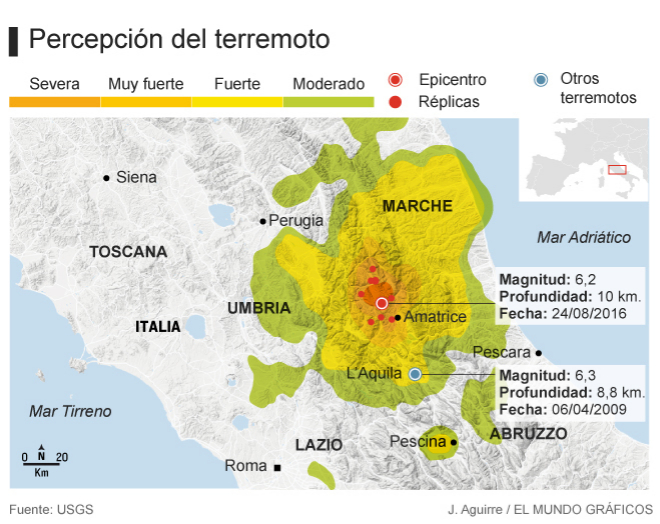
\includegraphics[height=7cm]{../imagenes/2_estado_del_arte/percepcion_terremoto_italia.jpg}
%\caption{Percepcion del terremoto en Italia en 2016. Fuente: \cite{MELGUIZO2016}}
%\end{figure}

\chapter{}

%---------------------------------------------------------
%	1.	Seccion
%---------------------------------------------------------

%\section{}


%\begin{figure}[hb] 
%\centering
%\subfigure[]{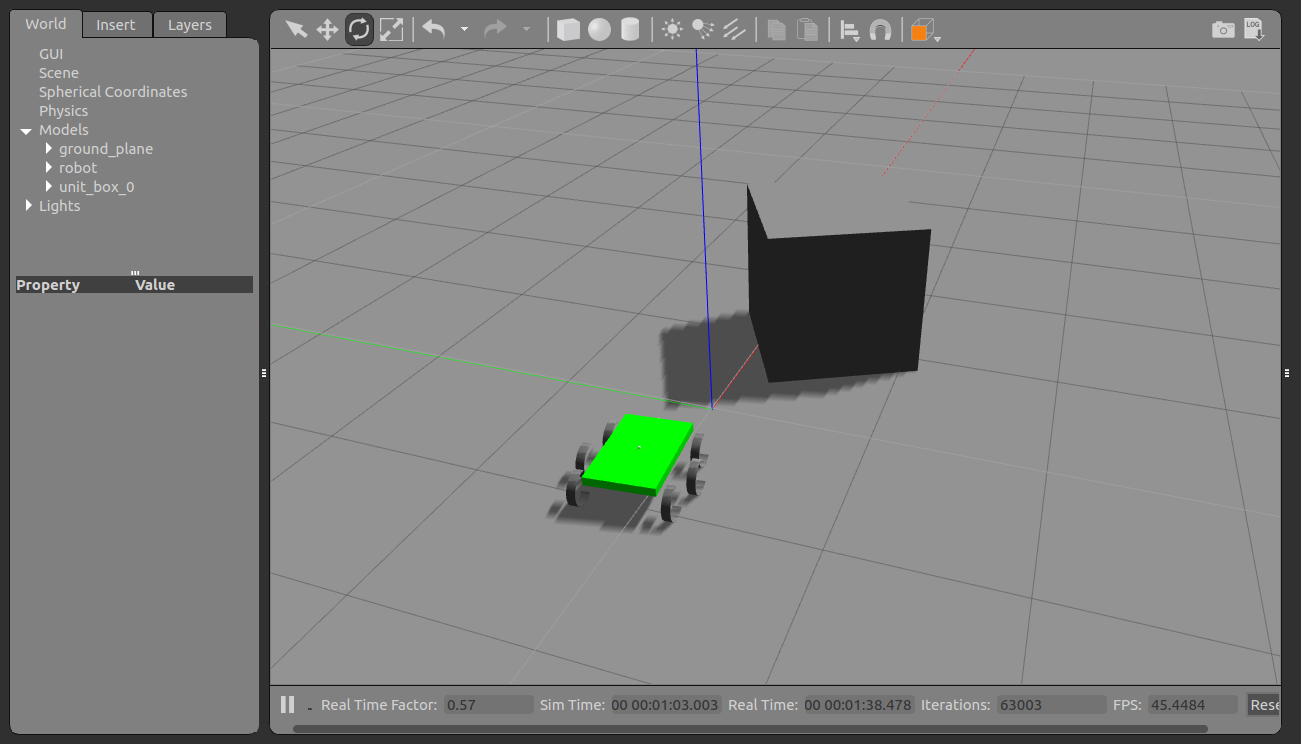
\includegraphics[width=0.9\textwidth]{../imagenes/3_modelado_rhex/rhex_sensor_1.png}}
%\subfigure[]{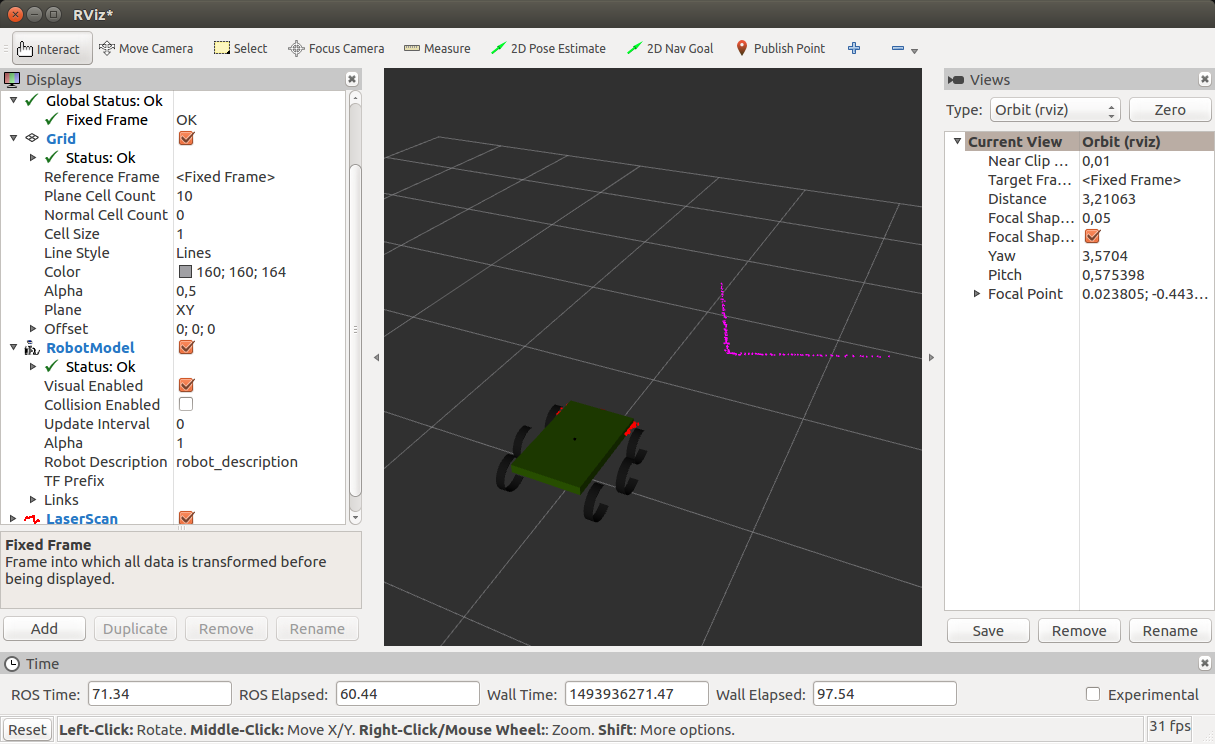
\includegraphics[width=0.9\textwidth]{../imagenes/3_modelado_rhex/rhex_sensor_2.png}}
%\caption{Información captada por el Hokuyo ante un obstáculo.}
%\label{fig:hokuyo_obs}
%\end{figure}
%#########################################################
%	Documento
%#########################################################

\chapter{}

\chapter{}


\chapter{}


\chapter{Conclusiones y líneas futuras.}

%--------------------------------------------------------
%	1.	
%--------------------------------------------------------

\section{Conclusiones.}


%---------------------------------------------------------
%	Anexos
%---------------------------------------------------------

%\appendix
\renewcommand\appendixname{Anexo}
\chapter{}



%---------------------------------------------------------
%	Bibliografía
%---------------------------------------------------------

%Estilo bibliografia
\bibliographystyle{acm}
%Archivo bibliografia
%\bibliography{../DB_bibliografia/bib_tfg_raul_cebolla_13069}

\end{document}